\subsubsection{usergoal-ugGetMissionInRange}

\label{RE-use-case-ugGetMissionInRange}


The actVolunteer's goal is to retrieve help requests that are in a specific range 		  


\begin{usecase}
  \addheading{Use-Case Description}
  \addsingletwocolumnrow{Name}{ugGetMissionInRange}
  \addsingletwocolumnrow{Scope}{system}
  \addsingletwocolumnrow{Level}{usergoal}
  

\addrowheading{Primary actor(s)}
\addnumberedsinglerow{}{\msrcode{actVolunteer[active]}}


\addrowheading{Secondary actor(s)}
\addnumberedsinglerow{}{\msrcode{actPositionRequester[]}}
\addnumberedsinglerow{}{\msrcode{actSensor[]}}

\addrowheading{Goal(s) description}
\addsinglerow{The actVolunteer's goal is to retrieve help requests that are in a specific range }


\addrowheading{Protocol condition(s)}
\addnumberedsinglerow{}{The system has been deployed.
}

\addrowheading{Pre-condition(s)}
\addnumberedsinglerow{}{
}

\addrowheading{Main post-condition(s)}
\addnumberedsinglerow{}{The system returns a non null list of HelpRequest or a message indicating that none has been found within the specified range
}

\addrowheading{Main Steps}
\addalphanumberedsinglerow{}{the actor \msrcode{actPositionRequester} executes the \msrucname{oeGetPositionFromSensor} use case}
\addalphanumberedsinglerow{}{the actor \msrcode{actSensor} executes the \msrucname{oeSendPos} use case}
\addalphanumberedsinglerow{}{the actor \msrcode{actVolunteer} executes the \msrucname{oeGetInRangeMission} use case}

\addrowheading{Additional Information}
\addsinglerow{
none
}

\end{usecase} 


Figure \ref{fig:lu.uni.lassy.excalibur.g01.specification-RE-UCD-uc-ugGetMissionInRange}
User goal Get mission in range

\begin{figure}[htbp]
\begin{center}

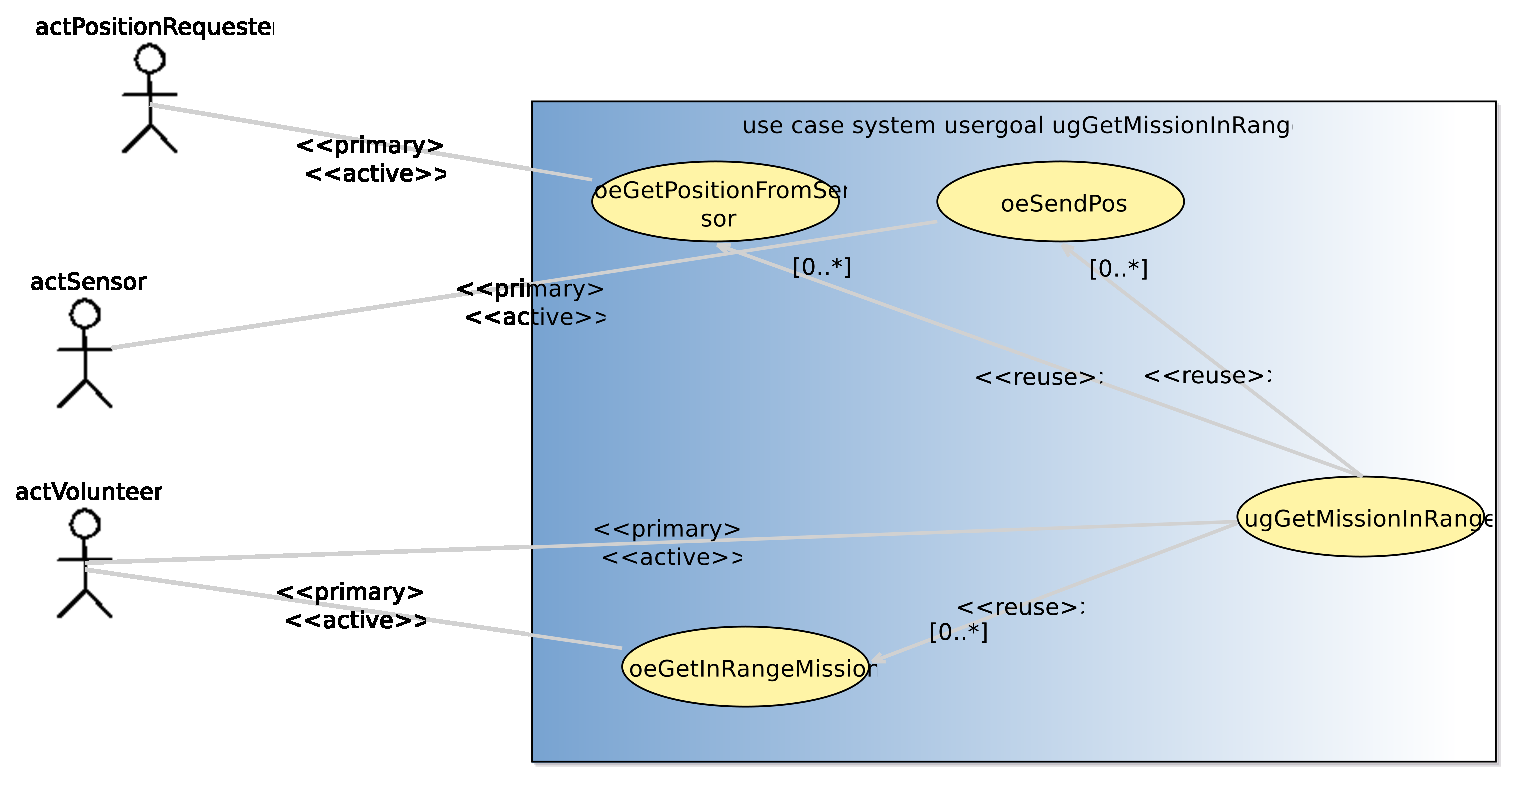
\includegraphics[
angle=0
]{./images-report-gen/usecase-model/usergoal/uc-ugGetMissionInRange.eps}
\end{center}
\caption[lu.uni.lassy.excalibur.g01.specification Use Case Diagram: uc-ugGetMissionInRange]{}
\label{fig:lu.uni.lassy.excalibur.g01.specification-RE-UCD-uc-ugGetMissionInRange}
\end{figure}
\vspace{0.5cm}
